
\documentclass[12pt]{article}
\setlength\parindent{0pt}
\usepackage{fullpage}
\usepackage[margin=0.5in, paperwidth=13.5in, paperheight=8.4in]{geometry}
\usepackage{amsmath}
\usepackage{graphicx}
\setlength{\parskip}{4mm}
\def\LL{\left\langle}   % left angle bracket
\def\RR{\right\rangle}  % right angle bracket
\def\LP{\left(}         % left parenthesis
\def\RP{\right)}        % right parenthesis
\def\LB{\left\{}        % left curly bracket
\def\RB{\right\}}       % right curly bracket
\def\PAR#1#2{ {{\partial #1}\over{\partial #2}} }
\def\PARTWO#1#2{ {{\partial^2 #1}\over{\partial #2}^2} }
\def\PARTWOMIX#1#2#3{ {{\partial^2 #1}\over{\partial #2 \partial #3}} }
\newcommand{\BE}{\begin{displaymath}}
\newcommand{\EE}{\end{displaymath}}
\newcommand{\BNE}{\begin{equation}}
\newcommand{\ENE}{\end{equation}}
\newcommand{\BEA}{\begin{eqnarray}}
\newcommand{\EEA}{\nonumber\end{eqnarray}}
\newcommand{\EL}{\nonumber\\}
\newcommand{\la}[1]{\label{#1}}
\newcommand{\ie}{{\em i.e.\ }}
\newcommand{\eg}{{\em e.\,g.\ }}
\newcommand{\cf}{cf.\ }
\newcommand{\etc}{etc.\ }
\newcommand{\Tr}{{\rm tr}}
\newcommand{\etal}{{\it et al.}}
\newcommand{\OL}[1]{\overline{#1}\ } % overline
\newcommand{\OLL}[1]{\overline{\overline{#1}}\ } % double overline
\newcommand{\OON}{\frac{1}{N}} % "one over N"
\newcommand{\OOX}[1]{\frac{1}{#1}} % "one over X"



\begin{document}
\pagenumbering{gobble}
\Large
\centerline{\sc{Recitation Questions -- Angular Momentum}}

\normalsize
\centerline{\sc{April 9}}

Recall that the angular momentum $L$ of an object can be found two ways:

$$L = I \omega \text{ (an object rotating around its center)}$$

or

$$L = mv_\perp r = mvr_\perp \text{ (a separate object moving past an object that can rotate)}$$

This second formula is best understood in words:

$$ L = \text{(mass of separate object)} \times \text{(radius from that object to the axis of rotation)} \times \text{(the component of the object's velocity perpendicular to the radius)} $$

or

$$ L = \text{(mass of separate object)} \times \text{(velocity of that object)} \times \text{(the component of the vector from the center of rotation to the object which is perpendicular to the velocity)} $$
\bigskip\bigskip



Conservation of ordinary momentum (``linear momentum'', $\vec p$) is most useful to understand collisions and explosions.

\bigskip

However, a rotating object can change its moment of inertia. This means that conservation of angular momentum is also useful when a rotating object changes its distribution of mass.

\newpage

\begin{enumerate}

	\item Consider the demo you saw in class: a person stands on a platform that is free to rotate. They are initially not rotating. You can approximate the person as a cylinder (with radius $r_p$ and mass $m_p$) in calculating their moment of inertia.
		Someone hands the person a horizontal bicycle wheel of radius $r_w$ of mass $m_w$ that is rotating clockwise rapidly around its vertical axis at angular velocity $\omega_0$.

		\begin{enumerate}
			\item When the person turns the bicycle wheel over (so it is rotating counterclockwise as seen from above rather than clockwise, for instance), how quickly and in which direction will they begin to rotate?
\vspace{3in}
			\item In class, the bicycle wheel was filled with concrete; its mass was likely around $m_w = 5$ kg. Estimate $r_p$ and $m_p$ for an average person, and estimate $r_w$. Is your result for the final angular velocity of the person reasonable? {\it (The moment of inertia of a thin ring, like the wheel, is $MR^2$; the moment of inertia of a cylinder is $\frac{1}{2}MR^2$.)}
		\end{enumerate}
\newpage
	\item We return to our astronaut using a jet pack to maneuver in space. {\it (This question, and the next one, are on HW7.)}

		\begin{minipage}{0.6\textwidth}

			
		Several engineers are debating how to design this jet pack:

			\bigskip

		{\bf Alex:} We're making a rocket, right? We just need one jet that can spit out gas. Let's build a backpack and put the gas exhaust in the middle of the astronaut's back. Gas comes out their back, astronaut goes forward, easy!

\bigskip

		{\bf Beth:} Don't do that -- then they can't go backwards! We need to put one in the back and one in the front, one behind their back pointing backwards and one in front of their stomach pointing forwards.

\bigskip

		{\bf Charlie:} Wait. Don't we need them to be able to turn around, too?

\bigskip

		They settle on this design -- a backpack worn by the astronaut with a horizontal bar sticking out from their hips, with four thrusters on the ends of the bar. These thrusters are capable of emitting puffs
		of gas at 300 m/s; each one is located 60 cm off to the side.
		\end{minipage}
		\begin{minipage}{0.3\textwidth}
			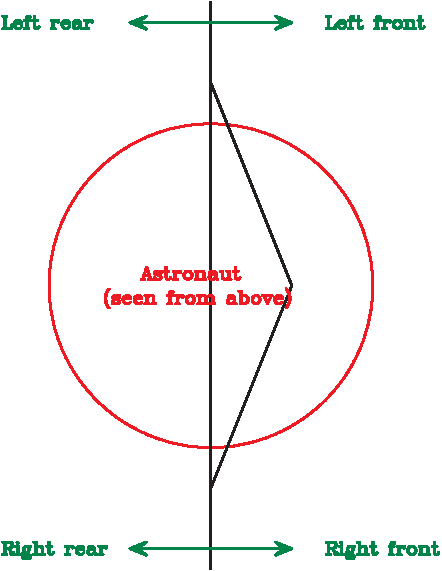
\includegraphics[width=0.9\textwidth]{jetpack-crop.pdf}
		\end{minipage}
		\begin{enumerate}
			\item Why does this design need {\it four} thrusters, off center, to allow the astronaut to maneuver? {\it (Reference the conservation of angular momentum in your explanation.)}
			
			\vspace{0.5in}
			
			\item If the astronaut wishes to accelerate forward, without rotating, which thrusters should they fire?
			
						\vspace{0.5in}
			\item If the astronaut fires the left rear thruster by itself, how will their velocity change? What about their angular velocity?
			
						\vspace{0.5in}
			
			\item Suppose the astronaut doesn't want to accelerate, but just wants to generate a clockwise angular velocity. Which thrusters should they fire?
		\end{enumerate}
		\newpage
		
			\item An astronaut wearing this design of jetpack is floating in space, conducting a repair on a satellite, when someone throws them a 20 kg tool at 1 m/s. However, they throw it to the side; the astronaut must reach 
				their arm one meter to the left to catch the tool. 

				\begin{enumerate}
					\item Explain why the astronaut begins to rotate counterclockwise and why they begin to move backwards after they catch the tool.
					
					\vspace{1in}
					
					\item What will the astronaut's angular velocity and what will their velocity be after they catch it?
					
					\vspace{2in}
					
					\item If the astronaut has a mass of 200 kg, and their mass distribution can be approximated by a cylinder of radius 20 cm, how fast will they be rotating?
					
					\vspace{2in}
					
					\newpage
					
					\item They would like to use this jetpack to stop themselves from rotating. Which thrusters should they fire, and how much gas should they release from each one? {\it (Remember that the thrusters are 60 cm from the center.)}
					
					\vspace{3in}
					
					\item What will their velocity be after this maneuver? What should the astronaut do if they want to reduce their velocity back to zero?
				\end{enumerate}




\end{enumerate}
\end{document}
